
\section{Modeling Probabilistic Dynamic Systems}
In this section, we introduce the different models and techniques that will constitute the basis for representing and computing probabilistic trace alignments.

\subsection{Stochastic Workflow Nets}\label{subsec:spn}
As customary in probabilistic conformance checking \cite{DBLP:conf/bpm/LeemansSA19,DBLP:conf/icpm/PolyvyanyyK19,DBLP:journals/tosem/PolyvyanyySWCM20}, we adopt stochastic Petri nets \cite{MarsanCB84,Desel1998,RoggeSoltiAW13} as the underlying formal basis to represent processes. More specifically, we consider an interesting class of stochastic Petri nets with only immediate transitions (i.e., no timed ones), namely untimed Stochastic Workflow Nets (\uswn for short).
We assume to have a set $\alphabet = \tasks \cup \set{\tau}$ of labels, where labels in $\tasks$ indicate process tasks, whereas $\tau$ indicates an invisible execution step ($\tau$-transition). A \emph{trace} is a finite sequence of labels from $\tasks$.

\begin{definition} An \emph{untimed Stochastic Workflow Net (\uswn)}
is a tuple $\net = (P,T,F,\ell,W)$ where:
\begin{compactitem}
\item $(P,T,F)$ is a standard \emph{workflow net} with places $P$, transitions $T$, and flow relation $F$ such that there is exactly one \emph{input place} with no incoming arc, and exactly one \emph{output place} with no outgoing arcs;
\item $\ell: T \rightarrow \alphabet$ is a \emph{labeling function} mapping each transition $t \in T$ into a label $\ell(t) \in \alphabet$ - this either indicates the task executed upon firing $t$, or the fact that $t$ is an invisible transition (in the latter case, $\ell(t) = \tau$);
\item $W\colon T\to \mathbb{R}^+$ is a \emph{weight function} assigning a positive firing weight to each transition of the net.
\end{compactitem}
\end{definition}
Given an \uswn $\net$, we use dot notation to extract its constitutive components (e.g., $\net.P$ denotes its places). \emph{The same dot notation will be used for the other structures introduced in the paper}. We also use $\net.in$ and $\net.out$ to respectively denote the input and output place of $\net$.

As usual, the current state of execution is captured using a marking of the net, that is, a multiset over places $P$ indicating how many tokens populate each place.
%As pointed out above, \emph{we always assume, as customary in BPM, that the input \uswn is \underline{bounded}}, that is, in every state the number of tokens associated to each place cannot exceed a maximum, fixed threshold.
The notions of transition enablement and firing are also the standard ones, since they do not depend on the weight function, which provides the basis for capturing the stochastic behavior of the net. We use the following notation: given a marking $\marking$ over \uswn $\net$, we denote by $\enaset{\marking}{\net}$ the set of enabled transitions in $\marking$; given transition $t \in \enaset{\marking}{\net}$, we write $\fire{\marking}{t}{\marking'}{\net}$ to capture the fact that, within $\net$, firing $t$ in $\marking$ results in the new marking $\marking'$. A \emph{firing sequence of $\net$ starting from marking $\marking_0$} is a sequence $t_1\cdots t_n$ of transitions from $\net.T$ so that for every $i \in \set{1,\ldots,n}$, we have that $\fire{\marking_{i-1}}{t_i}{\marking_{i}}{\net}$. We say that the firing sequence results in $\marking_{n}$.

As customary in workflow nets, we consider two special markings: the \emph{input} (resp.~\emph{output}) marking $m_{in}^\net$ (resp.~$m_{out}^\net$) that assigns a single token to the input (resp.~output) place $\net.in$ (resp.~$\net.out$) of $\net$, and no token elsewhere. A \emph{valid sequence} $\seq = t_1\cdots t_n$ of $\net$ is a firing sequence of $\net$ starting from $m_{in}^\net$ and resulting in $m_{out}^\net$. A sequence of labels $\run = \alpha_1 \cdots \alpha_n$ from $\alphabet$ is a \emph{run} of $\net$ if there exists a valid underlying sequence $\seq = t_1\cdots t_n$ of $\net$  such that, for every $i \in \set{1,\ldots,n}$, we have $\net.\ell(t_i) = \alpha_i$. Run $\run$ may have different underlying valid sequences in $\net$, which we collectively refer to as $\seqs{\run}{\net}$. A trace $\trace$ is a \emph{model trace} of $\net$ (or $\net$-trace for short) if there exists an underlying run $\run$ of $\net$ that corresponds to $\trace$ once all occurrences of $\tau$ are removed. There may be multiple runs underlying a $\net$-trace $\trace$, and we collectively refer to them as $\runs{\trace}{\net}$. Finally, we denote the (possibly infinite) set of $\net$-traces as $\traces{\net}$.
\begin{example}
\label{ex:net}
  Figure~\eqref{fig:spn} shows an example of \uswn with input place $p_1$ and output place $p_7$. One run of the net is $\const{\tau c \tau a a \tau}$, which corresponds to trace $\const{caa}$. Overall, the net supports infinitely many finite traces of the form (represented using regular expressions):
\begin{inparaenum}[\it (i)]
\item $\const{aa^*}$,
\item $\const{cb}$,
\item $\const{caa^*}$.
\end{inparaenum}
\end{example}

When executing an \uswn, the crucial addition to the standard execution semantics of workflow nets is that, being the net stochastic, in each marking the set of enabled transitions gets associated to a discrete probability distribution. This is defined as follows: given a marking $\marking$ of $N$ and an enabled transition $t \in \enaset{\marking}{\net}$, the \emph{firing probability} of $t$ in $\marking$ is $\probt{t}{\marking}{\net} = \frac{\net.W(t)}{\sum_{t'\in \enaset{\marking}{\net}}\net.W(t')}$. As required, the probabilities associated to all enabled transitions in a marking always add up to 1.

Using firing probabilities as a basic building block, we define the probability $\prob{\seq}{\net}$ of a valid sequence $\seq = t_1\cdots t_n$ of $\net$ as the product of the probabilities associated to each transition: $\prob{\seq}{\net} = \prod_{i \in \set{1,\ldots,n}}\prob{t_i}{\marking_{i-1}}{\net}$. %For a run $\run$ of $\net$, its probability $\prob{\seq}{\net}$ is then obtained by summing up the probabilities of all valid sequences corresponding to $\run$: $\prob{\run}{\net} = \sum_{\seq \in \seqs{\run}{\net}} \prob{\seq}{\net}$. Likewise, for a trace $\trace$ of $\net$, its probability is obtained by summing up
For a trace $\trace$ of $\net$, its probability $\prob{\trace}{\net}$ is then obtained by collecting all its underlying runs, in turn collecting all their underlying valid sequences, summing up their respective probabilities: $\prob{\trace}{\net} = \sum_{\run \in \runs{\trace}{\net}} \sum_{\seq \in \seqs{\run}{\net}} \prob{\seq}{\net}$. This corresponds to the intuition that, to observe $\trace$, one can equivalently pick any of its underlying valid sequences. Notably, if a trace is not an $\net$-trace (i.e., it does not conform with $\net$), then its probability is 0. For convenience, when needed we represent an $\net$-trace as a pair $\tup{\trace,\prob{\trace}{\net}}$ where the probability assigned to $\trace$ by $\net$ is retained.
\begin{example}
  \label{ex:trace}
Consider the \uswn \net of Example~\ref{ex:net}. Considering trace $\const{caa}$, it is easy to see that it has only one underlying run, namely $\const{\tau c \tau a a \tau}$, in turn produced by a single underlying valid sequence. The firing probability of picking the first $\tau$-transition starting from the input marking is $1$, as there are no alternatives. In the new marking, where only one token is assigned to $p_2$, the firing probability of choosing the $\tau$-transition above is $\rho_{23} = \frac{v_{\tau_2}}{v_{\tau_2}+v_c}$, whereas that of choosing the $c$-transition below is $\rho_{24} = \frac{v_c}{v_{\tau_2}+v_c}$. Upon choosing the transition below, the new marking assigns only to $p_4$ one token, leaving just one choice to continue by moving that token to $p_6$. In that marking, the probability of choosing the $a$-transition above is $\rho_{65} = \frac{v_{a_3}}{v_{a_3}+v_b}$, resulting in the token being moved to $p_5$. In this new marking, the probability of iterating over the $a$-transition above is $\rho_{55} = \frac{v_{\tau_3}}{v_{\tau_3}+v_{a_2}}$, while that of completing in the output marking via the enabled $\tau$-transition is $\rho_{57} = \frac{v_{\tau_3}}{v_{\tau_3}+v_{a_2}}$. Hence, all in all $
  \prob{\const{caa}}{\net} = 1 \cdot \rho_{24} \cdot 1 \cdot \rho_{65} \cdot \rho_{55} \cdot \rho_{57}$.
\end{example}

By interpreting concurrency by interleaving, we can represent all transition firings of an \uswn, together with their probabilities, in a reachability graph.

\begin{definition}
The \emph{Reachability Graph} $\rg{\net}$ of \uswn \net is a triple $(M,E,P)$ where:
\begin{compactitem}[$\bullet$]
\item $M$ is the set of all reachable markings from $\marking_0^\net$ (including $\marking_0^\net$ itself).
\item $E \subseteq M \times \alphabet \times M$ is a $\alphabet$-\emph{labeled transition relation} induced by $\net$, that is, for $\marking,\marking' \in M$, we have edge $(\marking,a,\marking') \in E$ if and only if there exists transition $t$ in $\net$ with label $\ell(t) = a$ and such that $\fire{\marking}{t}{\marking'}{\net}$.
\item $P:E \rightarrow [0,1]$ is the \emph{transition probability} function assigning to each transition $(\marking,a,\marking') \in E$ its corresponding probability, obtained from the firing probability of the \uswn transition(s) that lead from $\marking$ to $\marking'$ and are labeled by $a$: $P(\marking,a,\marking') = \sum_{t_i \in \enaset{\marking}{\net} \text{ s.t.~} \net.\ell(t) = a \text{ and } \fire{\marking}{t}{\marking'}{\net}} \prob{t}{\marking}{\net}$.
\end{compactitem}
\end{definition}
Notice that, in the definition, we have to account for the possible case where, in a given state, distinct net transitions with the same label produce the same consequent state. In this case, they are indistinguishable when observing the execution traces of the net, and in fact they collapse into a single edge of the reachability graph. This is why, in this case, we accumulate all their firing probabilities into a single value.


In the remainder of the paper, given an \uswn $\net$, we always assume that it satisfies two structural assumptions that are natural in the BPM setting:
\begin{compactitem}
\item $\net$ is \emph{bounded}, that is, every marking in $\rg{\net}$ assigns at most a pre-defined number of tokens to each place;
\item $\rg{\net}$ does not contain loops where all edges are labeled with $\tau$.
\end{compactitem}
The first assumption indicates that a case of the process does not generate unboundedly many parallel threads, and guarantees in turn that the reachability graph contains finitely many states. The second assumption naturally corresponds to how $\tau$-transitions are used when modeling business processes, where they are essential in representing gateways (such as exclusive and parallel splits/joins), cascaded gateways without tasks in between, and skippable tasks.  In all these cases, multiple $\tau$-transitions may be used, but never creating completely invisible loops. Under this assumption, $\net$ enjoys a very interesting property: given a trace $\trace$, there are only boundedly many valid sequences that can produce it. Hence, the probability of a $\trace$ can be computed by:
\begin{inparaenum}[\it (i)]
\item exhaustively enumerating all its valid sequences;
\item calculating the probability of each such sequence;
\item summing up all the so-obtained probabilities.
\end{inparaenum}
Figure~\eqref{fig:rg} shows an example of a reachability graph.




%Technically:
%\begin{compactitem}
%\item $P$ is a finite set of \textit{places}.
%\item $T$ is a finite set of \textit{transitions}, each of which is associate to a label. Each label either denotes a task executed upon transition firing, or indicates an invisible transition; in the latter case, we employ the special label $\varepsilon$.\footnotesize{This corresponds to the standard notion of $\tau$-transitions in Petri nets, but we use $\varepsilon$ since in the remainder of the paper $\tau$ is used to refer to an execution trace.}
%%to which we associate a label $\lambda(t)\in\Sigma$, where $\Sigma$ also includes the empty string\footnote{Given that we are going to denote the traces as $\tau$ and $t$ as the Petri net Transitions, we choose to denote the empty string as such instead of $\tau$ as in current literature from Petri nets.} $\varepsilon$.
%\item $F\subseteq (P\times T)\cup (T\times P)$ is the flow relation, representing arcs linking places to transitions and transitions to places.
%%to which we associate a \textit{firing cost} $\omega\colon F\to\mathbb{N}$.
%\item The initial place $i\in P$ has no ingoing edges ($\not\exists t\in T. (t,i)\in F$).
%\item The final place $f\in P$ has no outgoing edges ($\not\exists t\in T. (f,t)\in F$).
%\item $W\colon T\to \mathbb{R}^+_{>0}$ defines a \textit{firing weight} associated to each transition.
%\end{compactitem}

%A \textit{marking} is an assignment of a given amount of indistinguishable tokens to places described by a vector $M\colon P\to \mathbb{N}$. We say that a given transition $t$ is \textit{enabled} if $M(p)\geq 1$ for each ingoing $p$ to $t$ ($(p,t)\in F$). If such transition is enabled, then it can \textit{fire} a token. The \textit{enabling transitions} $E(M)$ for a given marking $M$ are all the $t$ reachable from $p$ ($(p,t)\in F$) with $M(p)\neq 0$ where $t$ is enabled. When $t$ can fire a token for a marking $M$, we can generate a novel marking $M'$ from $M$ by moving the tokens from the ingoing places towards the outgoing places as follows:
%\[\forall p\in P.\; M'(p)=M(p)-\mathbf{1}_{(p,t)\in F}+\mathbf{1}_{(t,p)\in F}\]
%We denote the transition from marking $M$ to marking $M'$ via an enabling $t$ as a relation $M\overset{t}{\to}M'$. We say that an \uswn with initial marking $M$ is $k$-\textit{bounded} if each of the markings $M'$ reachable from $M$, $M$ included, have $\forall p\in P.\; M(p)\leq k$\\

\begin{figure}[!t]
	\centering
	\subfloat[A sample \uswn. Labels are shown in green, invisible transitions in grey, and weights in magenta.]{\label{fig:spn}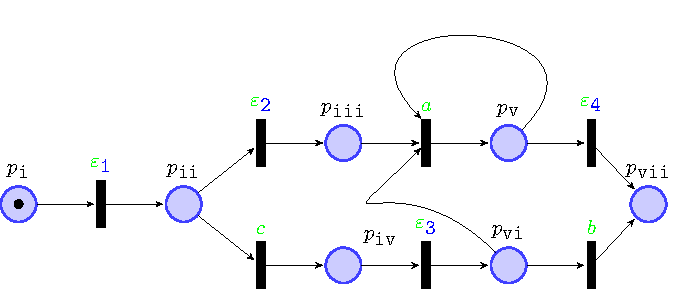
\includegraphics[width=.48\textwidth]{images/petri.pdf}}\hfill
    \subfloat[Reachability graph of the \uswn in (a). Probabilities are shown in violet.]{\label{fig:rg}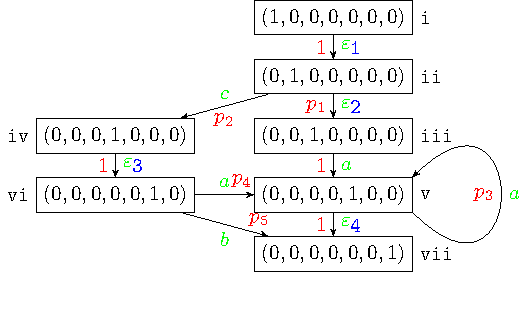
\includegraphics[width=.48\textwidth]{images/rg.pdf}}
    \\
\vspace*{-4.5mm}
	\subfloat[Transition graph encoding the reachability graph in (b).]{\label{fig:lmc}\label{fig:orig}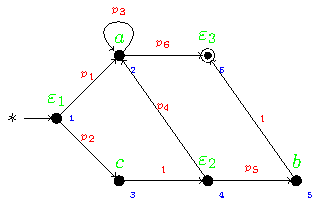
\includegraphics[width=.48\textwidth]{images/running_example.pdf}}
    \hfill
    \subfloat[Transition graph resulting from the transition graph in (c) after $\tau$-closure.]{\label{fig:closed}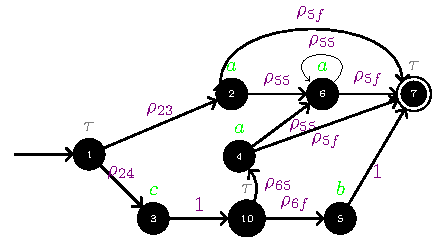
\includegraphics[width=.48\textwidth]{images/closed_example.pdf}}
	\caption{An \uswn and the application of the three transformation steps to convert it into a minimal, trace-preserving transition graph.}
	\label{transformspn}
\end{figure}
%Figures \ref{fig:spn} and \ref{fig:rg} respectively show a sample \uswn and its corresponding reachability graph. This net will be our running example throughout the paper.


%\begin{example}
%Figure \ref{fig:spn} provides a sample \uswn defined as such, and \ref{fig:rg} provides its associated Reachability Graph. This representation can be beneficial when such \uswns are inferred and extracted from log files \cite{PPNFromLog} for extracting the set of the probabilistic traces associated to the \uswn.
%\end{example}
%
%
%We use \uswns for modelling business processes: in fact, it can be shown \cite{RaedtsPUWGS07} that it is always possible to convert BPMNs to \uswns. Last, we also assume that a transition is enabled when all of its input places contain at least one token and that, when a transition fires, we remove one token from each of its input places and depose tokens for each of its output places.



\subsection{Transition Graphs}\label{subsec:ppn}

The graph and trace embedding techniques that we will use as the basis for computing probabilistic alignments cannot be directly defined over reachability graphs. In fact, these techniques rely on graphs where edges are only labeled by probabilities, whereas labels are attached to nodes. In addition, towards readily enabling efficient algorithmic techniques, such graphs are compactly defined using transition matrixes. We therefore take inspiration from \cite{GartnerFW03} and introduce the so-called \emph{probabilistic transition graphs}, which we will later use to encode \uswn{s} via their reachability graphs.

For a matrix $Q$ with row set $A$ and column set $B$, notation $[Q]_{ab}$ for $a \in A$ and $b \in B$ denotes the corresponding element in the matrix. In addition $\transp{Q}$ denotes the transposed matrix where rows and columns are inverted. We employ the usual sum and product operations over matrixes and arrays, and denote, for a square matrix $Q$, the repeated multiplication of $Q$ with itself $n$ times by $Q^n$.\todo{Rimuovere questo paragrafo se serve spazio,}\todo{NOn si capisce il significato di $\omega$}
%In our technical treatment, we continue to assume the existence of a set $\alphabet$ of labels (including the special label $\tau$).
\begin{definition} A \emph{(Probabilistic) Transition Graph} is a tuple $(V,s,t,L,R,\omega)$ where:
  \begin{inparaenum}[\itshape (i)]
    \item $V \subset \mathbb{N}$ is a set of \emph{nodes};
    \item $s\in V$ is the \emph{initial node};
    \item $e\in V$ is the \emph{accepting node};
    \item $L: \alphabet \times V \rightarrow \{0,1\}$ is a \emph{label matrix} associating each node in $V$ to a single label in $\alphabet$, where for label $\alpha \in \alphabet$ and node $\ind{i} \in V$, $[L]_{\alpha\ind{i}}$ gives $1$ if $\ind{i}$ is labeled by $\alpha$, $0$ otherwise;
    \item $R: V \times V \rightarrow [0,1]$ is a \emph{(probabilistic)} transition matrix indicating, for each pair of nodes, what is the probability that executing a transition from the first node leads to the second node;
    \item $\omega \in [0,1]$ is a \emph{graph weight} indicating an overall value associated to the entire graph.
  \end{inparaenum}
$L$ and $R$ satisfy the following well-formedness conditions:
\begin{inparaenum}[\itshape (i)]
\item for every $i \in V$ there is one and only one label $\alpha \in \alphabet$ so   that $[L]_{\alpha\ind{i}}=1$;
\item  for  every $\ind{i} \in V$, we have that $\sum_{\ind{j}\in V}[R]_{\ind{ij}}=1$.
\end{inparaenum}
\end{definition}
The condition for $L$ indicates that each node is mapped by $L$ to a single label, while the same label may be used for multiple nodes. The condition for $R$ ensures that the numbers contained therein can be interpreted as a probability distribution when choosing which next node to pick upon executing a transition.

A transition graph $\tg$ can be visualized as shown in Figures~\eqref{fig:lmc} and \eqref{fig:closed}. There, the various elements have the obvious interpretation, with the only important consideration that an edge from node $\ind{i}$ to node $\ind{j}$ is only shown if the transition probability $[\tg.R]_{\ind{i}\ind{j}}$ is positive.
%There, each node $\ind{i} \in \tg.V$ is  represented as a circle with its identifying number. The initial node is decorated by a small incoming edge, while the final node is double circled. The label of the node is shown close to the circle, in agreement with $\tg.L$. Finally, an edge from $\ind{i} \in \tg.V$ to $\ind{j} \in \tg.V$ is shown if the transition probability $[\tg.R]_{\ind{i}\ind{j}}$ is positive. Each edge is decorated with the positive probability assigned by $\tg.R$.

%\begin{definition}[Path, trace]
%A \emph{path} in a transition graph $\tg$ is a finite sequence of nodes $\ind{i}_1 \cdots \ind{i}_n$ (with $n > 1$) such that, for every $j \in \set{1,\ldots,n-1}$, we have that $[\tg.R]_{\ind{i}_j\ind{i}_{j+1}} > 0$. Such a path is \emph{valid} if it starts from the initial node and ends in the accepting node of $\tg$, that is, $\ind{i}_1 = \tg.s$ and $\ind{i}_n = \tg.e$.
%
%A \emph{trace} is a finite sequence of nodes that can be turned into a valid sequence by introducing in the sequence an arbitrary number of $\tau$ labels (so as to account for hidden transitions in the graph).
%\end{definition}
%From the definition, it is clear that every valid path can be straightforwardly converted into a corresponding trace by removing all $\tau$ labels from the sequence.

%$\npath{\ind{i}}{\ind{j}}$

By mirroring to definitions of \uswn{s} taking into account that now labels are on nodes, a \emph{valid sequence} of $\tg$ is a sequence $\ind{i}_0\ldots\ind{i}_n$ of nodes in $\tg.V$ that leads from the initial to the accepting node by only traversing transitions with nonzero probability:
\begin{inparaenum}[\it (i)]
\item $\ind{i}_0 = \tg.s$;
\item $\ind{i}_n = \tg.e$;
\item if the sequence contains at least two nodes, each two consecutive nodes are connected by a positive transition probability, i.e., for every $j \in \set{1,\ldots,n}$ we have $[R]_{\ind{i}_{j-1}\ind{i}_{j}} > 0$.
\end{inparaenum}
Runs and model traces of transition graphs are then defined as in \uswn{s}, and we employ the same notation to indicate the runs underlying a model trace, and the valid sequences underlying a run. The computation of probabilities for runs and traces is hence defined equivalently.

We close this section by introducing how some  matrix operations defined in the literature \cite{GartnerFW03} are applied to matrixes $L$ and $R$ of $\tg$, towards tackling interesting probability computations. These will be instrumental later on in the paper. Given two nodes $\ind{i},\ind{j} \in \tg.V$, $[R^n]_{\ind{i}\ind{j}}$ returns the probability of having a path in $\tg$ that connects $\ind{i}$ to $\ind{j}$ and has length $n$. Given two labels $\alpha,\beta \in \alphabet$, with $[LR^n\transp{L}]_{\alpha\beta}/[L\transp{L}]_{\alpha\alpha}$, we obtain the probability that, starting in any node labeled by $\alpha$, we reach a node labeled by $\beta$ through  $n$ consecutive steps in $\tg$. As a shortcut notation, we call the result $[\tg.\Lambda^n]_{\alpha\beta}$. Since there may be different nodes labeled by $\alpha$, we need to normalize the resulting probabilities. This is obtained with the division by $L\transp{L}$, which does so by assuming a uniform distribution when picking from which specific $\alpha$-labeled node one wants to start. Notice that these calculations need to be refined so as to consider proper runs and  traces. This will be done in Section~\ref{subsec:as}. %\todo{Rimandare alla sezione giusta}



%
%$\texttt{\color{blue}i}\overset{n}{\rightsquigarrow}\texttt{\color{blue}j}$ of length $n$: therefore, $[\Lambda^n]_{\color{green}\alpha\beta}:=[LR^nL^t]_{\color{green}\alpha\beta}/[LL^t]_{\color{green}\alpha\alpha}$ denotes the probability that, having started at any node labelled $\color{green}\alpha$ and taking $n$ steps, we arrive at any node labelled $\color{green}\beta$ (${\color{green}\alpha}\overset{n}{\rightsquigarrow}{\color{green}\beta}$). We denote as ${\color{green}\alpha}{\rightsquigarrow}{\color{green}\beta}$ an aforementioned path of arbitrary length.
%We can also associate a weight $\omega\in[0,1]\subseteq\mathbb{R}$ to a TG, so to express the probability associated with the TG itself as valid.
%




%\begin{example}
%We can graphically represent such TG as in \cite{Myers1989}.
%Figure \ref{fig:orig} is a  TG $P^*=(\mathtt{\color{blue}1},\mathtt{\color{blue}8},L,R,1)$ where $\omega=1$, where the matrices $L$ and $R$ can be both defined as follows:
%$$L:=\kbordermatrix{
%             & \texttt{\color{blue}1}&\texttt{\color{blue}2}&\texttt{\color{blue}3}&\texttt{\color{blue}4}&\texttt{\color{blue}5}&\texttt{\color{blue}6}&\texttt{\color{blue}7}&\texttt{\color{blue}8}&\texttt{\color{blue}9}&\texttt{\color{blue}10}\\
%\color{green}\varepsilon  & \textbf{1}&0&0&0&0&0&\textbf{1}&\textbf{1}&\textbf{1}&\textbf{1}\\
%\color{green}a            & 0&\textbf{1}&0&\textbf{1}&0&\textbf{1}&0&0&0&0\\
%\color{green}b            & 0&0&0&0&\textbf{1}&0&0&0&0&0\\
%\color{green}c            & 0&0&\textbf{1}&0&0&0&0&0&0&0\\
%}\qquad R:=\kbordermatrix{
%& \texttt{\color{blue}1}&\texttt{\color{blue}2}&\texttt{\color{blue}3}&\texttt{\color{blue}4}&\texttt{\color{blue}5}&\texttt{\color{blue}6}&\texttt{\color{blue}7}&\texttt{\color{blue}8}&\texttt{\color{blue}9}&\texttt{\color{blue}10}\\
%\texttt{\color{blue}1}  & 0&0&{\color{red}p_2}&0&0&0&0&0&{\color{red}p_1}&0\\
%\texttt{\color{blue}2}  & 0&0&0&0&0&{\color{red}p_3}&{\color{red}p_6}&0&0&0\\
%\texttt{\color{blue}3}  & 0&0&0&0&0&0&0&0&0&{\color{red}1}\\
%\texttt{\color{blue}4}  & 0&0&0&0&0&{\color{red}p_3}&{\color{red}p_6}&0&0&0\\
%\texttt{\color{blue}5}  & 0&0&0&0&0&0&0&{\color{red}1}&0&0\\
%\texttt{\color{blue}6}  & 0&0&0&0&0&{\color{red}p_3}&{\color{red}p_6}&0&0&0\\
%\texttt{\color{blue}5}  & 0&0&0&0&0&0&0&{\color{red}1}&0&0\\
%\texttt{\color{blue}8}  & 0&0&0&0&0&0&0&0&0&0\\
%\texttt{\color{blue}9}  & 0&{\color{red}1}&0&0&0&0&0&0&0&0\\
%\texttt{\color{blue}10}  & 0&0&0&{\color{red}p_4}&{\color{red}p_5}&0&0&0&0&0\\
%}$$
%\end{example}

% Given a TG $P=(s,t,L,R,\omega)$, a trace $\tau$ is a tuple in $(\Sigma\backslash\{\varepsilon\})^*$ denoting a path always originating from $s$ and terminating in $t$.


\subsection{Kernels and Trace Kernels}\label{subsec:katk}
As a foundational basis to compute trace alignments, we adapt similarity measures from the database literature.  Given a set of data examples $\mathcal{X}$, (e.g., string or traces, transition graphs) a (positive definite) \emph{kernel} function $k\colon \mathcal{X}\times \mathcal{X}\to \mathbb{R}$ denotes the similarity of elements in $\mathcal{X}$. If $\mathcal{X}$ is the $d$-dimensional Euclidean Space $\mathbb{R}^d$, the simplest kernel function is the inner product $\Braket{\mathbf{x},\mathbf{x}'}=\sum_{1\leq i\leq d}\mathbf{x}_i\mathbf{x}'_i$.
A kernel is said to \emph{perform ideally} \cite{Gartner03} when $k(x,x')=1$ whenever $x$ and $x'$ are the same object (\textit{strong equality}) and $k(x,x')=0$ whenever $x$ and $x'$ are distinct objects (\textit{strong dissimilarity}). A kernel is also said to be \emph{appropriate} when similar elements $x,x'\in\mathcal{X}$ are also close in the feature space. Notice that appropriateness can be only assessed  empirically \cite{Gartner03}.
A positive definite kernel induces a distance metric as \cite{Raedt}:
\begin{equation}\label{eq:dofk}
d_k(\mathbf{x},\mathbf{x}'):=\sqrt{k(\mathbf{x},\mathbf{x})-2k(\mathbf{x},\mathbf{x}')+k(\mathbf{x}',\mathbf{x}')}
\end{equation}
When the kernel of choice is the inner product, the resulting distance is the Euclidean distance $\norm{\mathbf{x}-\mathbf{x}'}{2}$. A normalized vector $\hat{\mathbf{x}}$ is defined as $\mathbf{x}/\norm{\mathbf{x}}{2}$. For a normalized vector we can easily prove that: $\norm{\hat{\mathbf{x}}-\hat{\mathbf{x}}'}{2}^2=2(1-\Braket{\hat{\mathbf{x}},\hat{\mathbf{x}}'})$.

When $\mathcal{X}$ does not represent directly a $d$-dimensional Euclidean space, we can use an \emph{embedding} $\embed\colon\mathcal{X}\to \mathbb{R}^d$ to define a kernel $k_\embed\colon \mathcal{X}\times \mathcal{X}\to\mathbb{R}$ as $k_\embed(x,x'):=\Braket{\embed(x),\embed(x')}$. As a result, $k_\embed(x,x')=k_\embed(x',x)$ for each $x,x'\in\mathcal{X}$.

The literature also provides a kernel representation for strings \cite{LodhiSSCW02,Raedt,GartnerFW03}, which we can directly employ for our traces. We now provide an intuition describing the desired features of this representation \cite{LodhiSSCW02}. If we associate each dimension in $\mathbb{R}^d$ to a different subtrace $\alpha\beta$ of size $2$ (i.e., $2$-grams\footnote{\label{fn:caveat}For our experiments, we choose to consider only $2$-grams, but any $p$-grams of arbitrary length $p\geq 2$ might be adopted \cite{Gartner03}. An increased size of $p$ improves precision but also incurs in a worse computational complexity, as it requires to consider all the arbitrary subtraces of length $p$ whose constitutive elements occur at any distance from each other within the trace.}), the associated coordinate should represent how frequently and ``compactly'' this subtrace is embedded in the trace $\trace$ of interest. Therefore, we introduce a \emph{decay factor} $\lambda\in[0,1]\subseteq\mathbb{R}$ that, for all $m$ subtraces where $\alpha$ and $\beta$ appear in $\trace$ at the same relative distance $L < |\trace|$, weights the resulting embedding as $\lambda^Lm$.

We need to lift this approach so as to consider all occurrences of subtraces $\alpha\beta$ at every distance between $1$ and $|\trace|-1$. To do so, we proceed in two steps. First, we encode $\trace$ into a ``linear'' transition graph $\tg_\trace$ (Figure~\ref{fig:taustar}) in the obvious way: \todo{Tagliare dopo i due punti se necessario.} each node in $G_\sigma.V$  corresponds to an element of the trace labeled correspondingly, and the nodes representing two consecutive elements in the trace are connected with a transition probability of 1 (whereas in all the other cases, the probability is 0). As a second step, we rely on the matrix operations introduced at the end of Section~\ref{subsec:ppn} to calculate a simplified version of the embedding defined in \cite{LodhiSSCW02,Raedt} as $\trembed_{\alpha\beta}(\trace)=\sum_{1\leq i\leq |\trace|}\lambda^i[(\tg_{\trace}.\Lambda)^i]_{\alpha\beta}$. \todo{No spazio per spiegare cosa succede...} This value can be seen as a reward.

The kernel between two traces corresponds to the sum of the products of such rewards calculated 2-gram by 2-gram for the two traces, namely \emph{kernel convolution} \cite{Haussler}. %\todo{L'ho provato a scrivere intuitivamente, ma non e' chiaro da dove arrivi questo modo di calcolarlo... deriva dalle formule sopra ma la digressione in mezzo e' lunga. Come possiamo fare per chiarire? L'esempio spiega bene tutto!}
This trace kernel returns strong dissimilarity when the two traces have no shared 2-grams at any arbitrary occurring length, but does not enjoy strong equality (as the similarity of a trace with itself is at least $\lambda^2$ - returned when the trace is a 2-gram).

%
%we can represent it as a TG \cite{Myers1989} $(1,{|\tau|},L_\tau,R_\tau,1)$ having $[L_\tau]_{{\color{green}\alpha}\texttt{\color{blue}i}}=1\Leftrightarrow \tau_{\texttt{\color{blue}i}}={\color{green}\alpha}$ and $[L_\tau]_{{\color{green}\alpha}\texttt{\color{blue}i}}=0$ otherwise, and $\forall i<|\tau|.\; [R_\tau]_{\texttt{\color{blue}i(i+1)}}=1 $ and $[R_\tau]_{\texttt{\color{blue}ij}}=0$ otherwise.
%Exploiting this encoding, we can adopt a simplified version of the embedding defined in \cite{LodhiSSCW02,Raedt} as $\embed_{\mathcal{T}}(\tau)_{{\color{green}\alpha\beta}}=\sum_{1\leq i\leq |\tau|}\lambda^i[(\Lambda_\tau)^i]_{\color{green}\alpha\beta}$.
%Please note that this definition is similar to a transition matrix embedding proposed in \cite{GartnerFW03} via geometric series, that is $\sum_i\lambda^i[R^i]_{\color{green}\alpha\beta}$.

\begin{figure}[!t]
	\centering
	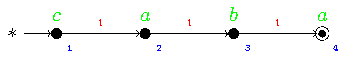
\includegraphics{images/taustar.pdf}
	\caption{Graphical representation of the transition graph encoding trace \const{cacb}}\label{fig:taustar}
\end{figure}
%
%\begin{example}\label{ex:tracembed}
%	{Let us suppose that we want to align a trace $\tau^*$ to one of the traces from a transition graph: in order to carry out an approximate alignment, we need to transform it to a transition graph first.} A trace $\tau^*=\textup{caba}$ can be graphically represented in Figure \ref{fig:taustar}. The associated TG $T=(\mathtt{\color{blue}1},\mathtt{\color{blue}4},L,R,1)$ has matrices $L$ and $R$  defined as follows:
%	$$L:=\kbordermatrix{
%		& \texttt{\color{blue}1}&\texttt{\color{blue}2}&\texttt{\color{blue}3}&\texttt{\color{blue}4}\\
%		\color{green}a            & 0&\textbf{1}&0&\textbf{1}\\
%		\color{green}b            & 0&0&\textbf{1}&0\\
%		\color{green}c            & \textbf{1}&0&0&0\\
%	}\qquad R:=\kbordermatrix{
%		& \texttt{\color{blue}1}&\texttt{\color{blue}2}&\texttt{\color{blue}3}&\texttt{\color{blue}4}\\
%		\texttt{\color{blue}1}  & 0&\color{red}1&0&0\\
%		\texttt{\color{blue}2}  & 0&0&\color{red}1&0\\
%		\texttt{\color{blue}3}  & 0&0&0&\color{red}1\\
%		\texttt{\color{blue}4}  & 0& 0& 0& 0\\
%	}$$
%We can similarly represent all the traces from the USPN.
%\end{example}

%\begin{example}
%The subtrace \textit{\textbf{\uline{hi}}} is represented in \textit{\textbf{\uline{hi}}deous},   \textit{\uline{\textbf{h}}e\uline{{i}}d\textbf{i}}, and \textit{\uline{{\textbf{h}i}}nd\textbf{i}}, but with different frequencies and subtrace distances. We have $\embed_{\mathcal{T}}(\textit{hideous})_{{\color{green}hi}}=\lambda$,  $\embed_{\mathcal{T}}(\textit{heidi})_{{\color{green}hi}}=\lambda^2+\lambda^4$, and $\embed_{\mathcal{T}}(\textit{hindi})_{{\color{green}hi}}=\lambda+\lambda^4$.
%\end{example}



\begin{table}[!b]
\caption{Embedding of traces \const{cacb}, \const{caaa}, \const{caa} and \const{cb}.}\label{tb:embedding}
\begin{center}
	\begin{tabularx}{\textwidth}{
>{\hsize=.1\hsize}X
>{\hsize=.2\hsize}X
>{\hsize=.1\hsize}X
>{\hsize=.1\hsize}X
>{\hsize=.1\hsize}X
>{\hsize=.1\hsize}X
>{\hsize=.1\hsize}X
>{\hsize=.25\hsize}X
>{\hsize=.2\hsize}X
>{\hsize=.1\hsize}X
}
		\toprule
		& $\const{aa}$    & $\const{ab}$   & $\const{ac}$    & $\const{ba}$   & $\const{bb}$   & $\const{bc}$ & $\const{ca}$ & $\const{cb}$ & $\const{cc}$   \\
		\midrule
		$\const{cacb}$ & $0$ & $\lambda^2$ & $\lambda$ & $0$  & $0$  & $0$ & $\lambda$ & $\lambda+\lambda^3$ & $\lambda^2$\\
		$\const{caaa}$ & $2\lambda+\lambda^2$& $0$ & $0$ & $0$ & $0$ & $0$ & $\lambda+\lambda^2+\lambda^3$ & $0$ & $0$ \\
		$\const{caa}$  & $\lambda$ & $0$ & $0$ & $0$ & $0$ & $0$ & $\lambda+\lambda^2$ & $0$&  $0$\\
		$\const{cb}$   & $0$ & $0$ & $0$ & $0$ & $0$ & $0$ & $0$ & $\lambda$& $0$ \\
		\bottomrule
	\end{tabularx}
\end{center}
\end{table}
\begin{example}\label{ex:wheredotiszero}
Consider tasks $\tasks=\Set{a,b,c}$. The possible 2-grams over $\tasks$ are $\tasks^2=\Set{\const{aa},\const{ab},\const{ac},\const{ba},\const{bb},\const{bc},\const{ca},\const{cb},\const{cc}}$. Table~\ref{tb:embedding} shows the embeddings of some traces. Being a 2-gram, trace $\const{cb}$ has only one nonzero component, namely that corresponding to itself, with $\trembed_{\const{cb}}(\const{cb})=\lambda$. Trace $\const{caa}$ has the 2-gram $\const{ca}$ occurring with length $1$ ($\const{\underline{ca}a}$) and $2$ ($\const{\underline{c}a\underline{a}}$), and the 2-gram $\const{aa}$ with occurring length $1$ ($\const{c\underline{aa}}$). Hence: $\trembed_{\const{ca}}(\const{caa})=\lambda+\lambda^2$ and  $\trembed_{\const{aa}}(\const{caa})=\lambda$.  Similar considerations can be carried out for the other traces in the table.

We now want to compute the similarity between the first trace $\const{cacb}$ and the other three traces. To do so, we sum, column by column (that is, 2-gram by 2-gram) the product of the embeddings for the two traces (thus keeping penalties whenever the 2-gram embeds in both traces). We then get
{\footnotesize
\[
k_{\trembed}(\const{cacb},\const{caaa})=\lambda(\lambda+\lambda^2+\lambda^3)
~~
k_{\trembed}(\const{cacb},\const{caa})=\lambda(\lambda+\lambda^2)
~~
k_{\trembed}(\const{cacb},\const{cb})=\lambda(\lambda+\lambda^3)
\]}
which induces ranking $
k_{\trembed}(\const{cacb},\const{caaa})>
k_{\trembed}(\const{cacb},\const{caa})>
k_{\trembed}(\const{cacb},\const{cb})
$.
\end{example}

\endinput
\subsection{Graph Embedding}\label{ssec:ge}
Graph kernels allow mapping graph data structures to feature spaces (usually an Eulcidean space in $\mathbb{R}^n$ for $n\in \mathbb{N}_{>0}$) \cite{Samatova} so to express graph similarity functions that can then be adopted for both classification \cite{TsudaS10} and clustering \cite{Raedt} algorithms. One of the first approaches used in literature involved the definition of topological description vectors \cite{Sidere} for each graph in a graph database, for then defining the graph similarity function as an inner product of their associated vectors. One inconvenience of such a technique is that it is required to perform NP-complete subgraph isomorphisms among a collection of graphs. It has been already proved that the definition of a graph kernel function fully recognising the structure the graph always boils down solving such  NP-Complete problem \cite{GartnerFW03}, as exact embeddings generable in polynomial can be inferred just for loop-free Direct Acyclic Graphs \cite{BergamiBM20}.


Consequently, most recent literature focused on extracting relevant features of such graphs, that are then used to define a graph similarity function. The most common approach adopted in the kernel to extract such features is called \textit{propositionalization}: we might extract all the possible features (e.g., subsequences), and then define a kernel function based on the occurrence and similarity of these features \cite{Gartner03}.

%\section{LTL over Finite Traces and the Declare Framework}
%\label{sec:preliminaries}
%As a formal basis for specifying crisp (temporal) business constraints, we adopt the customary choice of Linear Temporal Logic over finite traces (\LTLf \cite{DeVa13,DDGM14}). This logic is at the basis of the well-known \declare \cite{PeSV07} constraint-based process modeling language.
%We provide here a gentle introduction to this logic and to the \declare framework.
%
%\subsection{Linear Temporal Logic over Finite Traces}
%
%$\LTLf$ has exactly the same syntax as standard $\LTL$, but, differently from $\LTL$, it interprets formulae over an unbounded, yet finite linear sequence of states. Given an alphabet $\Sigma$ of atomic propositions (in our setting, representing activities), an \LTLf formula $\varphi$ is built by extending propositional logic with temporal operators:
%\[\varphi ::= a \mid \lnot \varphi \mid \varphi_1\lor \varphi_2
% \mid \Next\varphi \mid \varphi_1\Until\varphi_2 \quad \text{ where $a \in \Sigma$.}\]
%
%
%%The semantics of \LTLf is given in terms of \emph{finite traces}
%%denoting finite, \emph{possibly empty}, sequences
%%$\tau=\tau_0,\ldots,\tau_n$ of elements from the alphabet $\Sigma$. The evaluation of a formula is done in a given state (i.e., position) of the trace.
%
%
%The semantics of \LTLf is given in terms of \emph{finite traces} denoting finite, \emph{possibly empty} sequences $\tau=\tup{\tau_0, \ldots, \tau_n}$ of elements of $2^\Sigma$, containing all possible propositional interpretations of the propositional symbols in $\Sigma$. In the context of this paper, consistently with the literature on business process execution traces, we make the simplifying assumption that in each point of the sequence, one and only one element from $\Sigma$ holds. Under this assumption, $\tau$ becomes a total sequence of activity occurrences from $\Sigma$, matching the standard notion of (process) execution trace. We indicate with $\tasks^*$ the set of all traces over $\tasks$. The evaluation of a formula is done in a given state (i.e., position) of the trace, and we use the notation $\tau,i\models \varphi$ to express that $\varphi$ holds in the position $i$ of $\tau$. We also use $\tau \models \varphi$ as a shortcut notation for $\tau,0\models\varphi$. This denotes that $\varphi$ holds over the entire trace $\tau$ starting from the very beginning and, consequently, logically captures the notion of \emph{conformance} of $\tau$ against $\varphi$. We also say that $\varphi$ is \emph{satisfiable} if it admits at least one conforming trace.
%
%%We start by giving an intuitive account of the resulting semantics. In the syntax above, operator $\Next$ denotes the \emph{next state} operator, and $\Next \varphi$ is true if $\varphi$ is true is true now if there exists a next state (i.e., the current state is not at the end of the trace), and in the next state $\varphi$ holds. Operator $\Until$ instead is the \emph{until} operator, and $\varphi_1\Until\varphi_2$ is true if $\varphi_1$ holds now and continues to hold until eventually, in a future state, $\varphi_2$ holds. From the given syntax we can derive the usual boolean operators $\land$ and $\rightarrow$, the two formulae $\true$ and $\false$, as well also additional temporal operators. We consider in particular the following three:
%%\begin{compactitem}[$\bullet$]
%%\item (eventually) $\Diamond \varphi = \true \Until \varphi$ is true if there is a future state where $\varphi$ holds;
%%\item (globally) $\Box \varphi = \neg \Diamond \neg \varphi$ is true if now and in all future sates $\varphi$ holds;
%%\item (weak until) $\varphi_1 \Wntil \varphi_2 = \varphi_1\Until\varphi_2 \lor \Box \varphi_1$ relaxes the until operator by admitting the possibility that $\varphi_2$ never becomes true, in this case by requiring that is true if $\varphi_1$ holds now and in all future states.
%%\end{compactitem}
%% To define the semantics formally, we denote the length of trace $\tau$ as $\length(\tau) =  n+1$.
%
%
%In the syntax above, operator $\Next$ denotes the \emph{next state} operator, and $\Next \varphi$ is true if there exists a next state (i.e., the current state is not at the end of the trace), and in the next state $\varphi$ holds. Operator $\Until$ instead is the \emph{until} operator, and $\varphi_1\Until\varphi_2$ is true if $\varphi_1$ holds now and continues to hold until eventually, in a future state, $\varphi_2$ holds. From these operators, we can derive the usual boolean operators $\land$ and $\rightarrow$, the two formulae $\true$ and $\false$, as well as additional temporal operators. We consider, in particular, the following three:
%\begin{compactitem}[$\bullet$]
%\item (eventually) $\Diamond \varphi = \true \Until \varphi$ is true if there is a future state where $\varphi$ holds;
%\item (globally) $\Box \varphi = \neg \Diamond \neg \varphi$ is true if now and in all future states $\varphi$ holds;
%\item (weak until) $\varphi_1 \Wntil \varphi_2 = \varphi_1\Until\varphi_2 \lor \Box \varphi_1$ relaxes the until operator by admitting the possibility that $\varphi_2$ never becomes true, in this case by requiring that $\varphi_1$ holds now and in all future states.
%\end{compactitem}
%%We write $\tau \models \varphi$ as a shortcut notation for $\tau,0\models \varphi$, and say that formula $\varphi$ is \emph{satisfiable}, if there exists a trace $\tau$ such that $\tau \models \varphi$.
%
%\begin{example}
%The $\LTLf$ formula $\Box(\activity{accept} \rightarrow \Diamond\activity{pay})$ models that, whenever an order is accepted, then it is eventually paid. The structure of the formula follows what is called \emph{response template} in \declare.
%\end{example}
%
%%Every $\LTLf$ formula $\varphi$ can be translated into a corresponding standard finite-state automaton $\aut_\varphi$ that accepts all and only those finite traces that satisfy $\varphi$ \cite{DeVa13,DDGM14}. Although the complexity of reasoning with $\LTLf$ is the same as that of $\LTL$, finite-state automata are much easier to manipulate in comparison with B\"uchi automata, which are necessary when formulae are interpreted over infinite traces.
%
%\subsection{Declare}
%\begin{table}[t]
\caption{Some \declare templates, their textual and graphical representation, the corresponding \LTLf formalization and the \LTLf formula capturing their complement (i.e., their logical negation).
\label{tab:constraints}}
\centering
\begin{adjustbox}{width=0.9\textwidth,center}
\begin{tikzpicture}
  \matrix[  nodes={node distance=\nodedist,minimum height=6mm},
            rectangle, draw,
            nodes in empty cells,
            row sep=2mm,column sep=3mm,
            very thick,
            column 1/.style={anchor=west,font=\footnotesize},
            column 2/.style={anchor=west,xshift=1mm,font=\footnotesize},
            column 3/.style={anchor=west,xshift=1mm,font=\footnotesize},
            column 4/.style={anchor=west},
            >=latex,->,
          ] (declarematrix) {
    \node {\textsc{text}};
    &
    \node[yshift=.5mm] {\textsc{notation}};
  &
    \node {\textsc{\LTLf\ formula ($\varphi$)}};
    &
    \node[yshift=.5mm] {\textsc{complement ($\neg\varphi$)}};
    \\
    \node {
      \begin{tabular}{@{}l@{}}
      \constraint{existence($\mathit{a}$)} \\
      \end{tabular}
    };
    &
    \node[smalltask,xshift=1.5mm] (a) {$\mathit{a}$};
    \node[taskfg,above=-1mm of a,xshift=-.3mm]{\footnotesize $1..\ast$};
    &
    \node {$\Diamond {a}$};
    &
    \node {$\Box \neg {a}$};

    \\
     \node {
      \begin{tabular}{@{}l@{}}
        \constraint{absence2($\mathit{a}$)}\\
      \end{tabular}
    };
    &
    \node[smalltask,xshift=1.5mm] (a) {$\mathit{a}$};
    \node[taskfg,above=-1mm of a,xshift=-.3mm]{\footnotesize $0..1$};

    &
    \node {$\neg \Diamond ({a} \land \Next \Diamond {a})$};
    &
    \node {$\Diamond ({a} \land \Next \Diamond {a})$};
    \\
    \node {
      \begin{tabular}{@{}l@{}}
        \constraint{response($\mathit{a}$,$\mathit{b}$)}
      \end{tabular}
    };
    &
    \node[smalltask,xshift=1.5mm] (a) {$\mathit{a}$};
    \node[above=-1mm of a,xshift=-.3mm]{\footnotesize $~$};
    \node[smalltask,right=\taskdist of a] (b) {$\mathit{b}$};
    \path[response,very thick] (a) -- (b);
    &
    \node {$\Box ({a} \rightarrow \Diamond {b})$};
    &
    \node {$\Diamond ({a} \land \Box \neg {b})$};
    \\
    \node {
      \begin{tabular}{@{}l@{}}
        \constraint{precedence($\mathit{a}$,$\mathit{b}$)}\\
      \end{tabular}
    };
    &
    \node[smalltask,xshift=1.5mm] (a) {$\mathit{a}$};
    \node[smalltask,right=\taskdist of a] (b) {$\mathit{b}$};
    \path[precedence,very thick] (b) -- (a);
    &
    \node {$\neg {b} \Wuntil {a}$};
    &
    \node {$\neg {a} \Until {b}$};
    \\
    \node {
      \begin{tabular}{@{}l@{}}
        \constraint{not-coexistence($\mathit{a}$,$\mathit{a}$)}\\

      \end{tabular}
    };
    &
    \node[smalltask,xshift=1.5mm] (a) {$\mathit{a}$};
    \node[smalltask,right=\taskdist of a] (b) {$\mathit{b}$};
    \path[notcoexistence,very thick] (a) -- (b);
    &
    \node {$\neg(\Diamond {a} \land \Diamond {b})$};
    &
    \node {$\Diamond {a} \land \Diamond {b}$};
    \\
%    \node {
%      \begin{tabular}{@{}l@{}}
%        \constraint{neg-response(\activity{a},\activity{b})}\\
%        $\Box( \activity{a} \limp \neg \bigcirc\Diamond \activity{b})$
%      \end{tabular}
%    };
%    &
%    \node[smalltask,xshift=1.5mm] (a) {\activity{a}};
%    \node[smalltask,right=\taskdist of a] (b) {\activity{b}};
%    \path[negationresponse,very thick] (a) -- (b);
%    \\
    };
\end{tikzpicture}
\end{adjustbox}
\end{table} 
%\declare\ \cite{PeSV07} is a declarative process modeling language based on \LTLf. More specifically, a \declare model fixes a set of activities, and a set of constraints over such activities, formalized using \LTLf formulae. The overall model is then formalized as the conjunction of the \LTLf formulae of its constraints.
%
%Among all possible \LTLf formulae, \declare selects some pre-defined patterns. Each pattern is represented as a \declare template, i.e., a formula with placeholders to be substituted by concrete activities to obtain a constraint. Constraints and templates have a graphical representation; Table~\ref{tab:constraints} lists the \declare templates used in this paper. A \declare model is then graphically represented by showing its activities, and the application of templates to such activities (which indicates how the template placeholders have to be substituted to obtain the corresponding constraint).
%
%%Automata-based techniques for $\LTLf$ have been adopted to tackle fundamental tasks within the lifecycle of \declare processes, such as consistency checking \cite{PeSV07,MPVC11}, enactment and monitoring \cite{PeSV07,MMWV11,DDGM14}, and discovery support \cite{MaCV12}.
%
%
%
%
%\begin{example}
%\label{ex:inconsistency}
%Consider the following \declare model, constituting a (failed) attempt of capturing a fragment of an order-to-shipment process:
%
%\begin{center}
%  \resizebox{3.2cm}{!}{
%        \begin{tikzpicture}
%        \node[task] (accept) {\accept};
%        \node[task,right=of accept] (reject) {\reject};
%        \node[left=0mm of accept,taskfg] {1..*};
%        \node[right=0mm of reject,taskfg] {1..*};
%        \draw[notcoexistence] (accept) -- (reject);
%    \end{tikzpicture}
%  }
%\end{center}
%
%The model indicates that there are two activities to accept or reject an order, that these two activities are mutually exclusive, and that both of them have to be executed.
%%  \begin{wrapfigure}[13]{l}{42mm}
%%  \end{wrapfigure}
%These constraints are obviously contradictory and, in fact, the model is inconsistent, since its \LTLf formula
%$
%\Diamond \accept \land \Diamond \reject \land \neg (\Diamond \accept \land \Diamond \reject)
%$
%is unsatisfiable.
%\end{example}
%
%
%
%\endinput
%
%\smallskip\noindent\textbf{\declare} is a constraint-based process modeling language based on \LTLf. Differently from imperative process modeling languages,
%\declare models a process by fixing a set of activities, and defining a set of
%\emph{temporal constraints} over them, accepting every execution trace that satisfies all constraints.
%Constraints are specified via pre-defined \LTLf templates, which come with a corresponding
%graphical representation (see Table~\ref{tab:constraints} for the \declare patterns we use in this paper).
%For the sake of generality, in this paper we consider arbitrary \LTLf formulae as constraints. However, in the examples we consider formulae whose templates can be represented graphically in \declare.
%
%
%
%Automata-based techniques for $\LTLf$ have been adopted in \declare to tackle fundamental tasks within the lifecycle of Declare processes, such as consistency checking \cite{PeSV07,MPVC11}, enactment and monitoring \cite{PeSV07,MMWV11,DDGM14}, and discovery support \cite{MaCV12}.
